\chapter{Qui}
\label{chap:qui}

\section{Quaraquaraqua}
\label{sec:quaqaraqua}

This is a reference to a chapter \ref{chap:quo}. This is a reference to a figure \ref{fig:doge}. This is a reference to some code \ref{lst:hello}. This is a citation \cite{famous:paper}.

\lstinputlisting[label=lst:hello, firstline=2, lastline=4, caption={I directly included a portion of a file}]{code/hello.py}

\begin{lstlisting}[language=Java, label=lst:java, caption={Some code in another language than the default one}]
public void prepare(AClass foo) {
  AnotherClass bar = new AnotherClass(foo)
}
\end{lstlisting}

\Blindtext


%    \usepackage{fullpage}
%    \usepackage{fourier}

\usetikzlibrary{calc,3d}

\thispagestyle{empty}

\begin{center}
  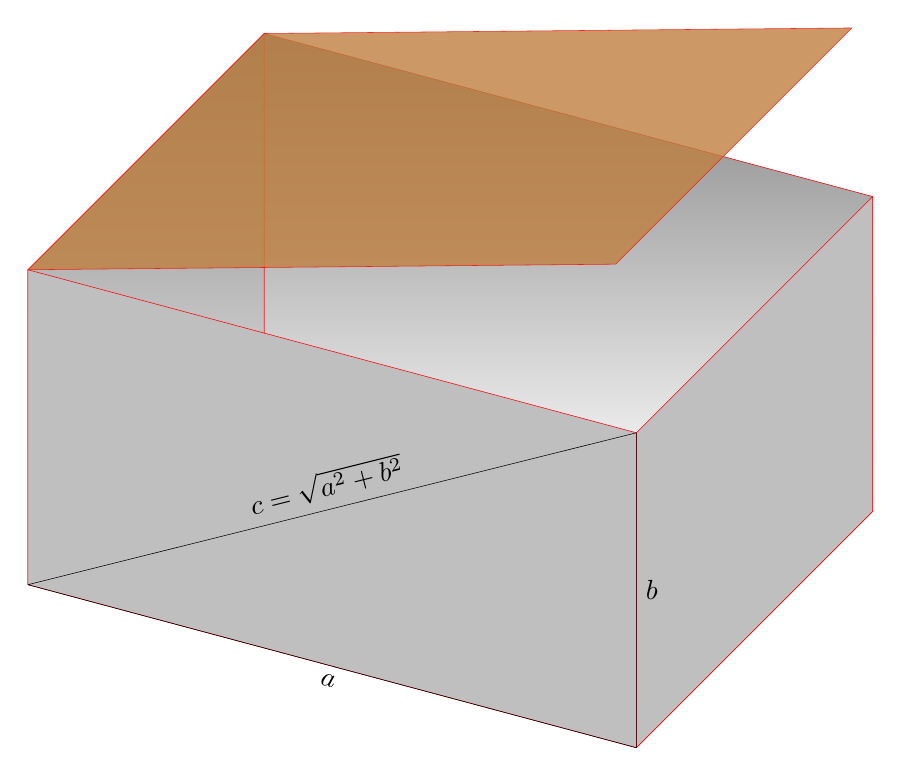
\begin{tikzpicture}[x  = {(-0.5cm,-0.5cm)},
    y  = {(0.9659cm,-0.25882cm)},
    z  = {(0cm,1cm)},
    scale = 2,
    color = {lightgray}]
    % style of faces
    \tikzset{facestyle/.style={fill=lightgray,draw=red,very thin,line join=round}}
    % face "back"
    \begin{scope}[canvas is zy plane at x=0]
      \path[facestyle,shade] (0,0) rectangle (2,4);
    \end{scope}
    % face  "left"
    \begin{scope}[canvas is zx plane at y=0]
      \path[facestyle,shade] (0,0) rectangle (2,3);
    \end{scope}
    % face "front"
    \begin{scope}[canvas is zy plane at x=3]
      \path[facestyle] (0,0) rectangle (2,4);
    \end{scope}
    % face  "right"
    \begin{scope}[canvas is zx plane at y=4]
      \path[facestyle] (0,0) rectangle (2,3);
    \end{scope}
    % face "up"
    \draw[fill=brown,draw=red,opacity=.8,very thin,line join=round]
    (0,0,2) --
    (3,0,2) --
    (3,{4*cos(15)},{4*sin(15)+2}) --
    (0,{4*cos(15)},{4*sin(15)+2}) --cycle ;
    % labels
    \draw[very thin,black,line join=round]
    (3,0,0) -- node [sloped,below] {$a$}
    (3,4,0) -- node [right]        {$b $}
    (3,4,2) -- node [sloped,above] {$c=\sqrt{a^2+b^2}$}
    (3,0,0);
  \end{tikzpicture}
\end{center}

\begin{figure}
  \begin{center}
    \includegraphics[width=0.5\columnwidth]{images/doge.png}
  \end{center}
  \caption{This is not a figure. It's a caption.}
  \label{fig:doge}
\end{figure}
